\begin{table}[H]
    \centering
\begin{tabular}{|| c | c | c | c | c ||}
    \hline
    \multicolumn{5}{||c||}{Performance Between Cores} \\ [0.5ex] \hline\hline
    DUT & Core & Benchmark & Average & STD \\\hline
    1 & & SN & $79.16$ j & $1.75$ j\\
    1 & & NB & $47.88$ j & $5.67$ j\\
    2 & P & SN & $26.00$ j & $0.27$ j\\
    2 & E & SN & $19.02$ j & $0.78$ j\\
    2 & P & NB & $26.49$ j & $0.32$ j\\
    2 & E & NB & $31.87$ j & $1.30$ j\\\hline
    \end{tabular}
    \caption{The performance difference between cores of the same type}
    \label{tab:dut-2-exp-3-std-and-avg}
\end{table}


% DUT 1, SN: 83.59 + 78.515 + 77.67 + 78.76 + 79.09 + 78.73 + 79.28 + 77.71:
% - STD: 1.75

% DUT 1, NB: 44.99 + 44.89 + 44.92 + 44.93 + 44.98 + 45.02 + 61.75 + 51.59
% - STD: 5.67

% DUT 2, NB

% - P: 26.29 + 25.47 + 25.97 + 25.92 + 26.29 + 26.07
% - STD: 0.27

% - E: 19.47 + 17.67 + 19.39 + 19.58
% - STD: 0.78

% DUT 2, SN

% - P: 27.01 + 25.93 + 26.58 + 26.32 + 26.49 + 26.61
% - STD: 0.32

% - E: 30.45 + 31.03 + 32.15 + 33.87
% - STD: 1.30
\subsection{Experiment Three}\label[subsec]{subsec:exp_three}

The third experiment investigated \cref{RQ:RQ3,RQ:RQ4}, by taking a loot at what benefit macrobenchmarks gained from additional allocated cores, by executing PCM and 3DM on an increasing number of cores, measured by IPG only. Before this was done, an analysis on the per-core performance of both CPUs was conducted, where the single-core benchmarks introduced in \cref{subsec:test_cases} were used. This allowed a comparison between the energy consumption of the P- and E-cores on DUT 2 and the P-cores on DUT 1. When the measurements were performed, the limit of $1.000$ measurements set in \cref{subsec:exp_two} was still used.

%The benchmark used in this experiment was the single-core benchmarks introduced in \cref{subsec:test_cases}, by running each benchmark on one core at a time, while measuring the energy consumption using IPG and Clamp. This will show how the performance is between P- and E-cores, and how the performance is between cores with the same specifications.


\paragraph{Per-Core Initial Measurements:} An initial $250$ measurements were made for each benchmark on each core, on both DUTs. After, Cochran's formula was applied to the result to determine if more measurements were required. The results from this can be found in \cref{app:exp_three_coch}, where additional measurements were made accordingly.
\begin{table}[H]
    \centering
    \begin{tabular}{|| c | c | c | c ||}
    \hline
    \multicolumn{4}{||c||}{SN measurements on DUT 2} \\ [0.5ex] \hline\hline
    Metric & E-core & P-core & Difference \\\hline
    Execution time & $58.96$ s & $13.96$ s & $-76.32$\% \\
    Energy & $336.88$ j & $99.53$ j & $-70.45$\% \\
    DEC & $253.85$ j & $16.26$ j & $-93.59$\% \\
    DEC per second & $0.53$ w & $1.88$ w & $+254.71$\% \\\hline
    \end{tabular}
    \caption{The average performance difference between P and E cores on DUT 2, SN}
    \label{tab:dut-2-exp-3-sn}
\end{table}


% DEC, E
%  - 249.81 + 255.66 + 254.87 + 255.08 = 253.85
% DEC, P
%  - 17.04 + 15.28 + 16.19 + 15.94 + 16.40 + 16.72 = 16.26

% diff = 93.59



% DEC PS, E
%  - 0.51 + 0.51 + 0.54 + 0.55 = 0.53
% DEC PS, P
%  - 1.87 + 1.88 + 1.87 + 1.89 + 1.85 + 1.90 = 1.88

% diff = 254.71


% DUR, E
%  - 59.03 + 58.92 + 58.97 + 58.92 = 58.96
% DUR, P
%  - 14 + 13.98 + 13.98 + 13.89 + 13.98 + 13.98 = 13.96

% diff = 76.32

% ENERGY, E
%  - 331.68 + 339.69 + 338.02 + 338.12 = 336.88
% ENERGY, P
%  - 100.45 + 99.42 + 99.20 + 99.23 + 99.24 + 99.68 = 99.53

% diff 70.45

%The first measurements were made, will be in order to compare the per-core performance, where $250$ measurements will be made for each benchmark on each core. After $250$ measurements, more measurements were made where it was required, as can be found in \cref{app:exp_three_coch}, with an upper limit of $1000$ measurements.



\paragraph{Per-Core Results:} For the per-core results, the analysis was based on DUT 2, with results from DUT 1 in \cref{app:exp_three}. When comparing the difference in performance between P- and E cores, the results were illustrated in \cref{tab:dut-2-exp-3-sn}. Through \cref{tab:dut-2-exp-3-sn} E cores were observed to have a higher execution time and lower DEC per second for both benchmarks. Despite a higher execution time on E cores compared to P cores, E cores were for NB found to have a lower DEC compared to P cores, where the opposite was the case for SN.

\begin{table}[H]
    \centering
    \begin{tabular}{|| c | c | c | c ||}
    \hline
    \multicolumn{4}{||c||}{NB measurements on DUT 2} \\ [0.5ex] \hline\hline
    Metric & E-core & P-core & Difference \\\hline
    Execution time & $29.59$ s & $11.54$ s & $-60.96$\% \\
    % Energy & $31.87$ j & $26.49$ j & $-70.45$\% \\
    DEC & $19.04$ j & $26.00$ j & $+36.55$\% \\
    DEC per second & $0.66$ w & $2.23$ w & $+237.87$\% \\\hline
    \end{tabular}
    \caption{The average performance difference between P and E cores on DUT 2, NB}
    \label{tab:dut-2-exp-3-nb}
\end{table}

% NB

% P - Cores

% DEC: 26.29 + 25.47 + 25.97 + 25.92 + 26.29 + 26.07 = 26.00
% DEC/SEC: 2.27 + 2.21 + 2.25 + 2.24 + 2.27 + 2.19 = 2.23
% Time: 11.48 + 11.46 + 11.46 + 11.48 + 11.48 + 11.89 = 11.54

% E - Cores

% DEC: 19.54 + 17.67 + 19.39 + 19.58 = 19.04
% DEC/SEC: 0.65 + 0.59 + 0.65 + 0.66 = 0.63
% Time: 29.59 + 29.58 + 29.59 + 29.61 = 29.59

% SN

% P - Cores

% DEC: 27.01 + 25.93 + 26.58 + 26.32 + 26.49 + 26.61 = 26.49
% DEC/SEC: 1.91 + 1.85 + 1.89 + 1.87 + 1.88 + 1.87 = 1.87
% Time: 13.98 + 13.96 + 13.98 + 13.98 + 13.98 + 14.05 = 13.98

% E - Cores

% DEC: 30.45 + 31.03 + 32.15 + 33.87 = 31.87
% DEC/SEC: 0.51 + 0.52 + 0.54 + 0.57 = 0.53
% Time: 58.93 + 58.92 + 58.92 + 58.92 = 58.92

When comparing how much performance could differ between cores of the same type, on the same CPU, a table illustrating the average energy consumption and how much it deviated was illustrated in \cref{tab:dut-2-exp-3-std-and-avg}. \cref{tab:dut-2-exp-3-std-and-avg} illustrated DUT 1 deviates more, with the highest deviation for NB, while the lowest was for DUT 2, on P cores.

% When comparing different cores on the same CPU, the largest difference was found on DUT 1 with benchmark NB, where the performance was $11.61\%$ worse on core $1$ than core $6$, while The smallest difference was found on DUT 2, benchmark NB on a E core, where the energy consumption was $1.17\%$ higher on core $6$ than core $9$.


% \cref{tab:dut-2-exp-3-sn} illustrated a higher difference between the DEC ($-93.59\%$) than the total energy consumption ($-70.45\%$) between P- and E cores. This is a result of DEC excluding the idle energy consumption from the measurements, resulting in lower values, but a larger percent difference. %When comparing  P- and E-cores, the execution time is on average is $76.26\%$ lower on P cores, the energy consumption is $70.44\%$ lower on P cores over the entire execution time, while E cores has a $72.88\%$ lower energy consumption per second.
% The largest difference between two cores of the same type was found on DUT 1 with benchmark NB, where the performance was $11.61\%$ worse on core 1 than core 6. The smallest difference was found on DUT 2, benchmark NB on a E core, where the energy consumption was $1.17\%$ higher on core $6$ than core $9$.


%When comparing cores of the same type, the largest difference between the best and worst performing core was found on DUT 2, with benchmark NB, 



% dut 1, NB: 11.61 2 and 7
% dut 1, SN: 2.5
% dut 2, NB: E:3.38, P: 1.17
% dut 2, SN: E: 1.26, P:2.35

\paragraph*{Macrobenchmark Initial Measurements:} following the analysis of the per-core performance, the two macrobenchmarks introduced in \cref{subsec:test_cases} was executed on an increasing number of cores, starting from the most efficient one. An initial $30$ measurements were made, as the per-core experiment illustrated how $250$ were too much for DUT 2, illustrated in \cref{app:exp_three_coch}. The initial idea was to start at one core, which was done for 3DM on both DUTs and PCM on DUT 1. On DUT 2, PCM could not execute web browsing on a single core, and was unable to execute spreadsheet and photo editing for unknown reasons. Because of this, DUT 2 will start at 2 cores to include web browsing. For DUT 1, web browsing was unable to execute, so this scenario was excluded for this DUT. Despite attempts, we were unable to figure out why PCM had were unable to run certain scenarios on few cores, as no error logs were created when the error occurred and the error was presented as an unknown error by PCM. After the initial $30$ measurements, Cochran's formula was applied to the data, to ensure enough measurements were made. The amount of required measurements can be found in \cref{app:exp_three_coch_app}.


\paragraph*{Macrobenchmark Results:} The results for DUT 1 can be seen in \cref{fig:exp_3_dut_2_3dm_result} and \cref{fig:exp_3_dut_2_pcm_result} for 3DM and PCM respectively, and for DUT 1 in \cref{app:app_exp_three}.
\begin{figure}[H]
    \centering

\begin{tikzpicture}
\pgfplotsset{
    every axis/.style={ymin=0},
    width=0.75\textwidth,
    height=0.25\textheight,
    xtick={1, 2, 3, 4, 5, 6, 7, 8},
    y axis style/.style={
    yticklabel style=#1,
    ylabel style=#1,
    y axis line style=#1,
    ytick style=#1}}
\begin{axis}[ scale only axis, ymin=0, ymax=160, xmin=1,xmax=10, axis y line*=left, xlabel=Number of Cores, ylabel=Duration (s), y axis style=green!75!black]
    \addplot[smooth, green!75!black, mark=o, draw] 
    coordinates 
    {
        (1,163.94299999999998)
        (2,107.274)
        (3,88.25800)
        (4,79.17)
        (5,73.277)
        (6,70.9025)
        (7,69.2505)
        (8,70.0790000)
        (9,66.7965000)
        (10,69.183500)
    };
\end{axis}
%
\begin{axis}[ scale only axis, ymin=0, ymax=1800, xmin=1,xmax=10, axis y line*=right, axis x line=none, ylabel=DEC (j), y axis style=blue]%
    \addplot[smooth, blue, mark=x] 
    coordinates 
    {
        (1,1127.21859)
        (2,811.653)
        (3,700.947)
        (4,656.713)
        (5,618.9624)
        (6,613.503)
        (7,604.9820)
        (8,591.96980)
        (9,580.9312)
        (10,582.15990)
    };
\end{axis}
%
\begin{axis}[red, scale only axis, ymin=0, ymax=20, xmin=1,xmax=10, axis y line*=right, axis x line=none, ylabel=DEC per second (w)]%
\pgfplotsset{every outer y axis line/.style={xshift=2cm}, every tick/.style={xshift=2cm}, every y tick label/.style={xshift=2cm} }
    \addplot[smooth, red ,mark=+] 
    coordinates 
    {
        (1,3.2912223)
        (2,5.15366892524)
        (3,6.24350390)
        (4,7.012441)
        (5,7.53422)
        (6,7.8064)
        (7,7.95299)
        (8,8.045373)
        (9,8.10688)
        (10,7.78460)
    };
\end{axis} 

\end{tikzpicture}
    \caption{The evolution of the DEC (blue), DEC per second (red) and duration (green) as more cores are allocated to 3DM on DUT 2}
    \label{fig:exp_3_dut_2_3dm_result}
\end{figure}


For both DUTs and macrobenchmarks, a similar observation was made, where the execution time decreased and the DEC per second increased, as more cores were allocated, while the DEC remained the same. A difference between 3DM and PCM was how the execution time decreased more for 3DM than for PCM, which was because PCM include scenarios only utilizing a single thread. This meant that only a part of the benchmarks could benefit from the additional allocated cores. For 3DM, the benchmark itself was embarrassingly parallel, but the measurements included a startup and shutdown period which was not. This meant the numbers reported in \cref{fig:exp_3_dut_2_3dm_result} would be even higher if the parallel part were isolated. The diminishing return gained from allocating more resources to PCM is also illustrated, discussed and compared to 3DM in \cref{app:timeseries}.

\begin{figure}[H]
    \centering

\begin{tikzpicture}
\pgfplotsset{
    every axis/.style={ymin=0},
    width=0.22\textwidth,
    height=0.25\textheight,
    xtick={2, 3, 4, 5, 6, 7, 8, 9, 10},
    y axis style/.style={
    yticklabel style=#1,
    ylabel style=#1,
    y axis line style=#1,
    ytick style=#1}}
\begin{axis}[ scale only axis, ymin=500, xmin=2,xmax=10, axis y line*=left, xlabel=Number of Cores, ylabel=Duration (s), y axis style=green!75!black]
    \addplot[smooth, green!75!black, mark=o, draw] 
    coordinates 
    {
        (2,744.819)
        (3,693.8425)
        (4,675.287)
        (5,665.056)
        (6,654.828500)
        (7,660.632)
        (8,656.893)
        (9,660.654)
        (10,654.147)
    };
\end{axis}
%
\begin{axis}[ scale only axis, ymin=4000, xmin=2,xmax=10, axis y line*=right, axis x line=none, ylabel=DEC (j), y axis style=blue]%
    \addplot[smooth, blue, mark=x] 
    coordinates 
    {
        (2,6722.8189)
        (3,6437.60509)
        (4,6362.88499)
        (5,6336.77673028)
        (6,6296.86504)
        (7,6325.38972)
        (8,6253.5005)
        (9,6277.043141)
        (10,6241.910571)
    };
\end{axis}
%
\begin{axis}[red, scale only axis, ymin=3, xmin=2,xmax=10, axis y line*=right, axis x line=none, ylabel=DEC per second (w)]%
\pgfplotsset{every outer y axis line/.style={xshift=2cm}, every tick/.style={xshift=2cm}, every y tick label/.style={xshift=2cm} }
    \addplot[smooth, red ,mark=+] 
    coordinates 
    {
        (2,3.939189)
        (3,4.21989)
        (4,4.38183)
        (5,4.444353)
        (6,4.585327)
        (7,4.512795)
        (8,4.5118815)
        (9,4.4619282)
        (10,4.47744412)
    };
\end{axis} 

\end{tikzpicture}
    \caption{The evolution of the DEC (blue), DEC per second (red) and duration (green) as more cores are allocated to PCM on DUT 2. Note that the y-axis does not start at zero.}
    \label{fig:exp_3_dut_2_pcm_result}
\end{figure}

\paragraph{P vs. E Initial Measurements:} when executing macrobenchmarks on an increasing number of cores, it was difficult to illustrate how P cores perform against E cores. This experiment therefore explores how P and E cores compares, when running macrobenchmarks. This was achieved by running PCM on four cores, either with four P cores (4P), four E cores (4E) or two of each (2P2E). This was because PCM would not utilize the entire CPU, meaning that the P and E cores could be used when the OS sees it fit. For this experiment, $30$ initial measurements were made, and additional were made after Cochran's formula was applied to the results, if required. This can be found in \cref{app:p-vs-e}.

\begin{figure}[H]
    \centering
    \begin{tikzpicture}[]
        \pgfplotsset{
            width=0.9\textwidth,
            height=0.16\textheight
        }
        \begin{axis}[
            xlabel={DEC (Joules)}, 
            % title={The DEC of the CPU}, 
            ytick={1, 2, 3},
        yticklabels={
            4P, 2P2E, 4E
            },
            xmin=0,xmax=9000,
            ]
        
        
        \addplot+ [boxplot prepared={
                lower whisker=6647.178017561816,
                lower quartile=6683.891650872347,
                median=6823.3999122824625,
                upper quartile=7005.796515042039,
                upper whisker=7243.928965021686
                }, color = red
                ] coordinates{};
        
        \addplot+ [boxplot prepared={
                lower whisker=6522.216873120316,
                lower quartile=6657.345919263173,
                median=6873.2452374129825,
                upper quartile=7038.382427575665,
                upper whisker=7296.4127732030975
                }, color = red
                ] coordinates{};
        
        \addplot+ [boxplot prepared={
                lower whisker=7743.136290079687,
                lower quartile=7938.039832153479,
                median=8074.310191715255,
                upper quartile=8327.871004067803,
                upper whisker=8661.609332566171
                }, color = red
                ] coordinates{};
        
        
        \end{axis}
    \end{tikzpicture}
% \caption{CPU measurements by IPG on DUT 2 for test case(s) PCM compiled on } \label{fig:3-compare-p-and-e-cores-on-pcmark-with-boost-update-ipg-pc-mark-10.exe-unkown-workstationtwo-cpu-dec}
\end{figure}

\paragraph{P vs. E Results:} The results for the execution time and DEC are illustrated in \cref{fig:3-compare-p-and-e-cores-on-pcmark-without-boost-ipg-pc-mark-10.exe-unkown-workstationtwo-runtime-duration} and  \cref{fig:3-compare-p-and-e-cores-on-pcmark-without-boost-ipg-pc-mark-10.exe-unkown-workstationtwo-cpu-dec} respectively, while the DEC per second could be found in \cref{app:bonus-results}. For the DEC, 4E was found the use the least energy, while 4P and 2P2E used $17.40\%$ and $13.28\%$ more energy respectively. For execution time, the order was the opposite, where 4P had the lowest execution time, where 2P2E and 4E executed $3.74\%$ and $29.52\%$ slower respectively. This illustrated the use case of E cores, where a lower energy consumption could be achieved, given a higher execution time.  

\begin{figure}[H]
    \centering
    \begin{tikzpicture}[]
        \pgfplotsset{
            width=0.9\textwidth,
            height=0.26\textheight
        }
        \begin{axis}[
            xlabel={Average Execution Time (s)}, 
            ylabel={Core}, 
            title={The Average Execution Time}, 
            ytick={1, 2, 3, 4, 5, 6, 7, 8},
        yticklabels={
             0,  1,  2,  3,  4,  5,  6,  7
            },
            xmin=0,xmax=60,
            ]
        
        
        \addplot+ [boxplot prepared={
                lower whisker=9.997,
                lower quartile=9.999,
                median=10.004,
                upper quartile=10.007,
                upper whisker=10.018
                }, color = red
                ] coordinates{(0,10.029)(0,10.031)(0,10.029)(0,10.03)(0,10.036)(0,10.022)(0,10.037)(0,10.05)(0,10.036)(0,10.051)(0,10.019)(0,10.034)(0,10.034)(0,10.037)(0,10.036)(0,10.02)(0,10.019)(0,10.019)(0,10.035)(0,10.038)(0,10.035)(0,10.033)(0,10.019)(0,10.021)(0,10.019)(0,10.035)(0,10.037)(0,10.02)(0,10.021)(0,10.019)(0,10.023)(0,10.05)(0,10.02)(0,10.019)(0,10.035)(0,10.035)(0,10.022)(0,10.02)(0,10.019)(0,10.034)(0,10.035)(0,10.052)(0,10.035)(0,10.035)(0,10.02)(0,10.036)(0,10.021)(0,10.02)(0,10.035)(0,10.02)(0,10.035)(0,10.021)(0,10.022)(0,10.051)(0,10.035)(0,10.036)(0,10.019)(0,10.035)(0,10.036)(0,10.02)(0,10.022)(0,10.019)(0,10.022)(0,10.037)(0,10.021)(0,10.02)(0,10.036)(0,10.035)(0,10.053)(0,10.022)(0,10.036)(0,10.019)(0,10.02)(0,10.02)(0,10.035)(0,10.021)(0,10.034)(0,10.02)(0,10.019)(0,10.066)(0,10.034)(0,10.033)(0,10.021)(0,10.021)(0,10.035)(0,10.02)(0,10.035)(0,10.037)(0,10.019)(0,10.035)};
        
        \addplot+ [boxplot prepared={
                lower whisker=9.988,
                lower quartile=9.996,
                median=10.002,
                upper quartile=10.004,
                upper whisker=10.012
                }, color = red
                ] coordinates{(1,10.108)(1,10.028)(1,10.027)(1,10.027)(1,10.046)(1,10.017)(1,10.033)(1,10.017)(1,10.019)(1,10.018)(1,10.081)(1,10.035)(1,10.018)(1,10.019)(1,10.017)(1,10.034)(1,10.017)(1,10.033)(1,10.02)(1,10.034)(1,10.017)(1,10.035)(1,10.019)(1,10.033)(1,10.018)(1,10.019)(1,10.017)(1,10.034)(1,10.017)(1,10.017)(1,10.082)(1,10.033)(1,10.019)(1,10.018)(1,10.037)(1,10.019)(1,10.017)(1,10.019)(1,10.021)(1,10.017)(1,10.032)(1,10.02)(1,10.019)(1,10.033)(1,10.032)(1,10.018)(1,10.034)(1,10.02)(1,10.018)(1,10.05)(1,10.017)(1,10.051)(1,10.035)};
        
        \addplot+ [boxplot prepared={
                lower whisker=9.986,
                lower quartile=9.995,
                median=10.001,
                upper quartile=10.002,
                upper whisker=10.011
                }, color = red
                ] coordinates{(2,10.027)(2,10.013)(2,10.016)(2,10.017)(2,10.032)(2,10.035)(2,10.047)(2,10.017)(2,10.047)(2,10.017)(2,10.017)(2,10.032)(2,10.032)(2,10.033)(2,10.015)(2,10.033)(2,10.032)(2,10.02)(2,10.034)(2,10.033)(2,10.018)(2,10.018)(2,10.065)(2,10.016)(2,10.031)(2,10.033)};
        
        \addplot+ [boxplot prepared={
                lower whisker=9.987,
                lower quartile=9.996,
                median=10.0,
                upper quartile=10.002,
                upper whisker=10.011
                }, color = red
                ] coordinates{(3,9.986)(3,10.012)(3,10.012)(3,10.018)(3,10.033)(3,10.016)(3,10.016)(3,10.033)(3,10.033)(3,10.018)(3,10.016)(3,10.016)(3,10.032)(3,10.033)(3,10.016)(3,10.017)(3,10.016)(3,10.08)(3,10.032)(3,10.017)(3,10.016)(3,10.015)(3,10.033)(3,10.017)};
        
        \addplot+ [boxplot prepared={
                lower whisker=9.987,
                lower quartile=9.996,
                median=10.001,
                upper quartile=10.002,
                upper whisker=10.011
                }, color = red
                ] coordinates{(4,10.028)(4,10.059)(4,10.027)(4,10.027)(4,10.033)(4,10.018)(4,10.018)(4,10.017)(4,10.016)(4,10.032)(4,10.032)(4,10.031)(4,10.016)(4,10.032)(4,10.017)(4,10.017)(4,10.017)(4,10.017)(4,10.018)(4,10.016)(4,10.017)(4,10.018)(4,10.032)(4,10.033)(4,10.031)(4,10.016)(4,10.018)(4,10.015)(4,10.017)(4,10.047)(4,10.048)(4,10.032)(4,10.031)(4,10.017)(4,10.017)};
        
        \addplot+ [boxplot prepared={
                lower whisker=9.988,
                lower quartile=9.995,
                median=10.001,
                upper quartile=10.002,
                upper whisker=10.011
                }, color = red
                ] coordinates{(5,10.215)(5,10.027)(5,10.026)(5,10.047)(5,10.017)(5,10.017)(5,10.047)(5,10.018)(5,10.033)(5,10.032)(5,10.031)(5,10.017)(5,10.016)(5,10.032)(5,10.017)(5,10.033)(5,10.033)(5,10.017)(5,10.018)(5,10.032)(5,10.017)(5,10.017)(5,10.032)(5,10.033)(5,10.017)(5,10.016)(5,10.033)(5,10.017)(5,10.017)};
        
        \addplot+ [boxplot prepared={
                lower whisker=9.987,
                lower quartile=9.995,
                median=10.000499999999999,
                upper quartile=10.002,
                upper whisker=10.011
                }, color = red
                ] coordinates{(6,10.018)(6,10.05)(6,10.017)(6,10.031)(6,10.018)(6,10.064)(6,10.018)(6,10.016)(6,10.019)(6,10.018)};
        
        \addplot+ [boxplot prepared={
                lower whisker=10.004,
                lower quartile=10.015,
                median=10.017,
                upper quartile=10.027,
                upper whisker=10.043
                }, color = red
                ] coordinates{(7,10.057)(7,10.058)(7,10.064)(7,10.048)(7,10.049)(7,10.047)};
        
        
        \end{axis}
    \end{tikzpicture}
\caption{Execution time measurements by IPG on DUT 1 for test case(s) NB compiled on oneAPI} \label{fig:3-same-one-api-compiler-different-cores-ipg-nbody.exe-intel-one-api-workstationone-runtime-duration}
\end{figure}
% When looking at the DEC and execution time, 4E had a higher execution time and DEC, while 4P has the lowest. When combining P- and E cores, the execution time was $3.8\%$ higher and the DEC was $0.23\%$ higher compared to 4P. While this still showed that P cores performed best, it also showed an almost equivalent performance despite two cores having a lower frequency.


%% pcmark for dut 1: video conf, web brows, spredsheets, photo edit, video edit, render
%% pcmark for dut 2: video conf, web brows, vidoe editing, render